% \iffalse
\let\negmedspace\undefined
\let\negthickspace\undefined
\documentclass[journal,12pt,twocolumn]{IEEEtran}
\usepackage{cite}
\usepackage{amsmath,amssymb,amsfonts,amsthm}
\usepackage{algorithmic}
\usepackage{graphicx}
\usepackage{textcomp}
\usepackage[justification=centering]{caption}
\usepackage{xcolor}
\usepackage{txfonts}
\usepackage{listings}
\usepackage{enumitem}
\usepackage{mathtools}
\usepackage{gensymb}
\usepackage{comment}
\usepackage[breaklinks=true]{hyperref}
\usepackage{tkz-euclide} 
\usepackage{listings}
\usepackage{gvv}                                        
\def\inputGnumericTable{}                                 
\usepackage[latin1]{inputenc}                                
\usepackage{color}                                            
\usepackage{array}                                            
\usepackage{longtable}                                       
\usepackage{calc}                                             
\usepackage{multirow}                                         
\usepackage{hhline}                                           
\usepackage{ifthen}                                           
\usepackage{lscape}
\newtheorem{theorem}{Theorem}[section]
\newtheorem{problem}{Problem}
\newtheorem{proposition}{Proposition}[section]
\newtheorem{lemma}{Lemma}[section]
\newtheorem{corollary}[theorem]{Corollary}
\newtheorem{example}{Example}[section]
\newtheorem{definition}[problem]{Definition}
\newcommand{\BEQA}{\begin{eqnarray}}
\newcommand{\EEQA}{\end{eqnarray}}
\newcommand{\define}{\stackrel{\triangle}{=}}
\theoremstyle{remark}
\newtheorem{rem}{Remark}
\begin{document}

\bibliographystyle{IEEEtran}
\vspace{3cm}

\title{10.5.3.9}
\author{EE23BTECH11063 - Vemula Siddhartha
}
\maketitle
\newpage
\bigskip

\renewcommand{\thefigure}{\theenumi}
\renewcommand{\thetable}{\theenumi}
\textbf{Question}:\\
If the sum of first 7 terms of an AP is 49 and that of 17 terms is 289, find the sum of
first n terms.
\\\\
\textbf{Solution: }\\
The sum of first $r$ terms of an Arithmetic Progression \brak{AP} $S_r$ , whose first term is $a$ and common difference is $d$ is:
\begin{align}
S_r=\frac{r}{2}\,\brak{2a+\brak{r-1}\,d}\label{eq10.5.3.9.1}
\end{align}
Let the given AP have first term $a$ and common difference $d$.\\
Given, the sum of first $7$ terms of the AP is 49.
\begin{align}
S_7&=49 \\
49&=\frac{7}{2}\,\brak{2a+\brak{7-1}\,d}  \\
49&=\frac{7}{2}\,\brak{2a+6d}  \\
a+3d&=7\label{eq10.5.3.9.2}
\end{align}
Also given, the sum of first $17$ terms of the AP is 289.
\begin{align}
S_{17}&=289  \\
289&=\frac{17}{2}\,\brak{2a+\brak{17-1}\,d}  \\
289&=\frac{17}{2}\,\brak{2a+16d}  \\
a+8d&=17 \label{eq10.5.3.9.3}
\end{align}
From  equations \ref{eq10.5.3.9.2} and \ref{eq10.5.3.9.3}:
\begin{align}
 \begin{pmatrix}
1&3\\
1&8
\end{pmatrix}  
\,
\begin{pmatrix}
    a\\
    d
\end{pmatrix}
&=
\begin{pmatrix}
    7\\
    17
\end{pmatrix}\\
\implies\begin{pmatrix}
    a\\
    d
\end{pmatrix}
&=
 \begin{pmatrix}
1&3\\
1&8
\end{pmatrix}^{-1}  
\begin{pmatrix}
    7\\
    17
\end{pmatrix}\\
\implies\begin{pmatrix}
    a\\
    d
\end{pmatrix}
&=
\frac{1}{5}\,
\begin{pmatrix}
    8&-3\\
    -1&1
\end{pmatrix}  
\begin{pmatrix}
    7\\
    17
\end{pmatrix}\\  
\implies\begin{pmatrix}
    a\\
    d
\end{pmatrix}
&=\frac{1}{5}\,
\begin{pmatrix}
    56-51\\
    -7+17
\end{pmatrix}\\  
\implies\begin{pmatrix}
    a\\
    d
\end{pmatrix}
&=
\begin{pmatrix}
    1\\
    2
\end{pmatrix}\\
\implies a=1&;\;d=2  
\end{align}

The sum of first n terms of the AP is:
\begin{align}
S_n= \frac{n}{2}\,\brak{2a+\brak{n-1}\,d}\label{eq10.5.3.9.4}
\end{align}
Substituting the values of $a$ and $d$:
\begin{align}
S_n&=\frac{n}{2}\,\brak{2\brak{1}+\brak{n-1}\brak{2}}  \\
S_n&=n\,\brak{1+n-1}  \\
S_n&=n^2\label{eq10.5.3.9.5}
\end{align}
The signal corresponding to this will be:
\begin{align}
    x\brak{n}= n^2\,u\brak{n}  
\end{align}

\begin{figure}[h]
    \renewcommand\thefigure{1}
    \centering
    \captionsetup{justification=centering}
    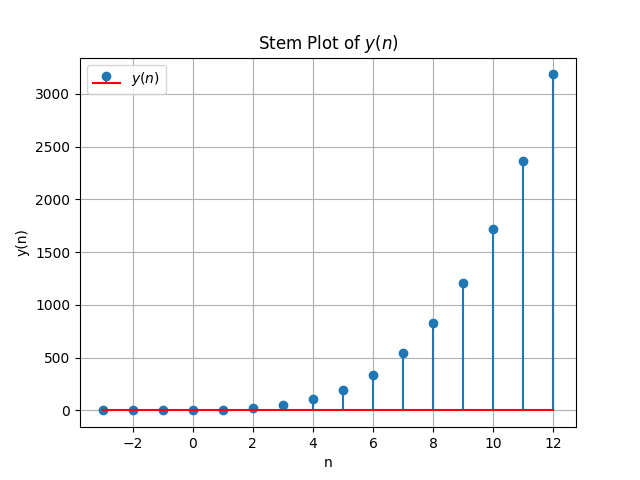
\includegraphics[width=1.1\linewidth]{Figure_1.png}
    \caption{Stem Plot of x(n)}
    \label{stemplot}
\end{figure}
Applying z-transform:
\begin{align}
X\brak{z}&=\sum_{n=-\infty}^{\infty}\brak{n^2\,u\brak{n}\,}z^{-n}  \\
X\brak{z}&=0+ \sum_{n=1}^\infty \brak{n^2}\,z^{-n}  
\end{align}
For the above series to converge, the limit of the modulus of the ratio of consecutive terms of the series must be less than 1:
\begin{align}
\implies\lim_{n\to\infty}\Bigg|\frac{\brak{n+1}^2\,z^{-\brak{n+1}}}{n^2\; z^{-n}}\Bigg|<1  
\end{align}
\begin{align}
&\implies\lim_{n\to\infty}\Bigg|\brak{\frac{n+1}{n}}^2\, z^{-1}\Bigg|<1  \\
&\implies\lim_{n\to\infty}\Bigg|\brak{1+\frac{1}{n}}^2\, z^{-1}\Bigg|<1  \\
&\implies|z|>\lim_{n\to\infty}\Bigg|\brak{1+\frac{1}{n}}^2\Bigg|  \\
&\implies|z|>1  
\end{align}
Hence, the Region of Convergence (ROC) is $|z|>1$.
\begin{align}
X\brak{z}&=\brak{1^2}\,z^{-1}+\brak{2^2}\,z^{-2}+\brak{3^2}\,z^{-3}+...  \\
X\brak{z}&=z^{-1}+4z^{-2}+9z^{-3}+16z^{-4}+...\label{eq10.5.3.9.6}
\end{align}
Multiplying the equation \ref{eq10.5.3.9.5} with $z^{-1}$:\\
\begin{align}
z^{-1}X\brak{z}&=z^{-2}+4z^{-3}+9z^{-4}+16z^{-5}+...\label{eq10.5.3.9.7}
\end{align}
Subtracting equation \ref{eq10.5.3.9.7} from equation \ref{eq10.5.3.9.6}:
\begin{align}
X\brak{z}\brak{1-z^{-1}}=z^{-1}+3z^{-2}+5z^{-3}+7z^{-4}+...\label{eq10.5.3.9.8}
\end{align}
Multiplying the equation \ref{eq10.5.3.9.7} with $z^{-1}$:
\begin{align}
X\brak{z}\brak{z^{-1}-z^{-2}}=z^{-2}+3z^{-3}+5z^{-4}+7z^{-5}+...\label{eq10.5.3.9.9}
\end{align}
Subtracting equation \ref{eq10.5.3.9.9} from equation \ref{eq10.5.3.9.8}:
\begin{align}
X\brak{z}\brak{1-2z^{-1}+z^{-2}}&=z^{-1}+2\brak{z^{-2}+z^{-3}+z^{-4}+...}  \\
X\brak{z}\brak{1-z^{-1}}^2&=z^{-1}+2\frac{\brak{z^{-2}}}{\brak{1-z^{-1}}}  \\
X\brak{z}&=\frac{z^{-1}\brak{1-z^{-1}}+2z^{-2}}{\brak{1-z^{-1}}^3}  \\
X\brak{z}&=\frac{z^{-1}\brak{1+z^{-1}}}{\brak{1-z^{-1}}^3}
\end{align}

Generalizing the problem:\\
Let the sum of first $n_1$ terms of the AP be 49, and the sum of first $n_2$ terms of the AP be 289.\\
From equation \ref{eq10.5.3.9.1}:
\begin{align}
\implies \frac{n_1}{2}\,\brak{2a+\brak{n_1-1}\,d}&=49\\
\implies a\brak{n_1}+ d\,\frac{\brak{n_1-1}\brak{n_1}}{2}&=49\label{eq10.5.3.9.10}
\end{align}
Also,
\begin{align}
\frac{n_2}{2}\,\brak{2a+\brak{n_1-1}\,d}&=289\\
\implies a\brak{n_2}+ d\,\frac{\brak{n_2-1}\brak{n_2}}{2}&=289\label{eq10.5.3.9.11}
\end{align}
From  equations \ref{eq10.5.3.9.10} and \ref{eq10.5.3.9.11}:
\begin{align}
    &\begin{pmatrix}
        n_1&\frac{\brak{n_1-1}\brak{n_1}}{2}\\
        n_2&\frac{\brak{n_2-1}\brak{n_2}}{2}
    \end{pmatrix}
    \begin{pmatrix}
        a\\
        d
    \end{pmatrix}
    =
    \begin{pmatrix}
        49\\
        289
    \end{pmatrix}
    \\
    &\begin{pmatrix}
        a\\
        d
    \end{pmatrix}
    =
    \begin{pmatrix}
        n_1&\frac{\brak{n_1-1}\brak{n_1}}{2}\\
        n_2&\frac{\brak{n_2-1}\brak{n_2}}{2}
    \end{pmatrix}^{-1}
    \begin{pmatrix}
        49\\
        289
    \end{pmatrix}
    \\
    &\begin{pmatrix}
        a\\
        d
    \end{pmatrix}
    =
    \frac{1}{n_1\brak{\frac{n_2^2-n_2}{2}}-\brak{\frac{n_1^2-n_1}{2}}n_2}
    \begin{pmatrix}
        \frac{n_2^2-n_2}{2} & \frac{-n_1^2+n_1}{2} \\
        -n_2 & n_1
    \end{pmatrix}
    \begin{pmatrix}
        49\\
        289
    \end{pmatrix}
    \\
    &\begin{pmatrix}
        a\\
        d
    \end{pmatrix}
    =
    \begin{pmatrix}
        \frac{-n_2+1}{n_1^2-n_1n_2} & \frac{-n_1+1}{n_2^2-n_1n_2} \\
        \frac{2}{n_1^2-n_1n_2} & \frac{2}{n_2^2-n_1n_2}
    \end{pmatrix}
    \begin{pmatrix}
        49\\
        289
    \end{pmatrix}
    \\
    \vspace{0.2cm}
    \implies &a=49\brak{\frac{-n_2+1}{n_1^2-n_1n_2}}+289\brak{\frac{-n_1+1}{n_2^2-n_1n_2}}\\
    \implies &d=49\brak{\frac{2}{n_1^2-n_1n_2}}+289\brak{\frac{2}{n_2^2-n_1n_2}}
\end{align}
 Substituting the values of a and d in the equation \ref{eq10.5.3.9.4}:
 \begin{align}
     \implies S_n = \frac{n}{2}\,\brak{2\brak{49\brak{\frac{-n_2+1}{n_1^2-n_1n_2}}}+289\brak{\frac{-n_1+1}{n_2^2-n_1n_2}}}\notag\\
     +\brak{n-1}\,\brak{49\brak{\frac{2}{n_1^2-n_1n_2}}+289\brak{\frac{2}{n_2^2-n_1n_2}}}
 \end{align}
 \begin{table}[h]
    \centering
    \renewcommand\thetable{1}
    \begin{tabular}[12.1pt]{ |c| c|}
    \hline
    \textbf{Variable} & \textbf{Description} \\ 
    \hline
    $a$ & First term of the AP \\
    \hline 
    $d$ & Common difference of the AP \\
    \hline
    $S_r$ & Sum of $r$ terms of the AP \\
    \hline
    $x(n)$ & General term \\
    \hline
    $X(z)$ & Z- transform of $x(n)$\\
    \hline    
    \end{tabular}
    \caption{Variables Used}
\end{table}
\end{document}  